\section{Beispiel 1: Spannungsstabilisierung mit Z-Diode}

\subsection{Dimensionierung von R1}

Zur Dimensionierung von R1 wurde die Schaltung zweimal parallel "aufgebaut". Einmal war dabei der Ausgang unbelastet, in der zweiten Schaltung wurde eine Stromsenke mit 3mA an den Ausgang geschaltet. Mit einem Parametric Sweep und einem Temperature Sweep wurde R1 variiert und f"ur die beiden Extremf"alle der Temperatur betrachtet (0 und 100 Grad).
Abbildung~\ref{fig:3_1_1_r1grob} zeigt den Verlauf der Abweichung der belasteten Ausgangsspannung vom unbelasteten Fall. Man erkennt, dass der 2\%-Punkt etwas "uber $1k\Omega$ liegt. Abbildung~\ref{fig:3_1_1_r1detail} zeigt diesen Bereich vergr"o\ss{}ert. Mit Cursors wurde der exakte Wert auf $1.1152k\Omega$ bestimmt (das ist der maximale Wert f"ur R1).

\begin{figure}%[h!]
	\centering
	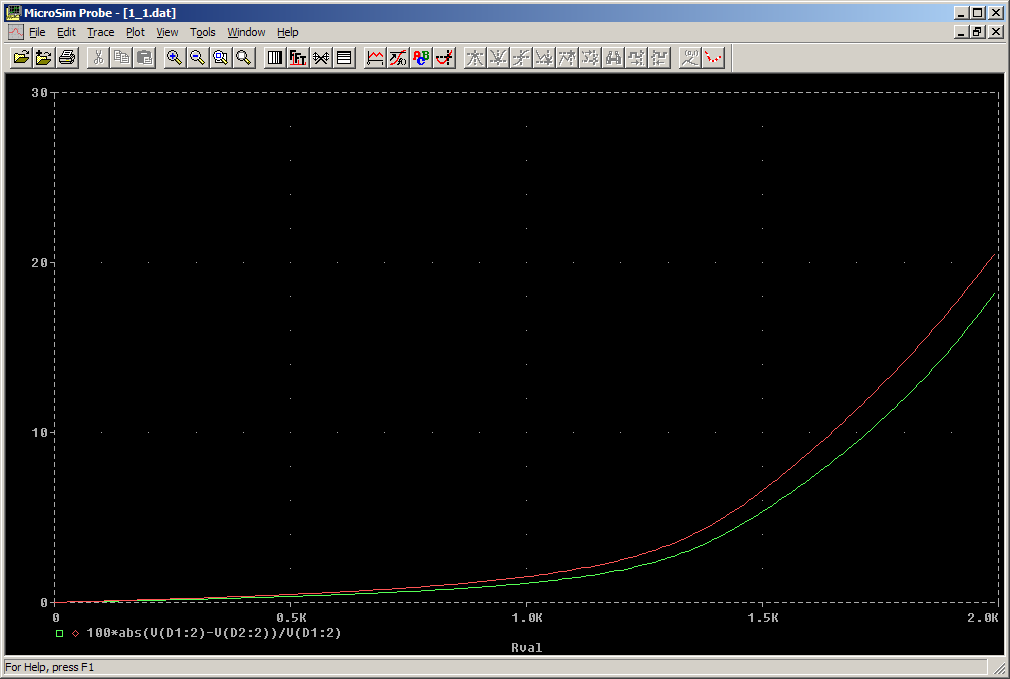
\includegraphics[width=\textwidth]{fig/bsp1/3_1_1_r1grob.PNG}
	\caption{Abweichung der Ausgangsspannungen f"ur grobe Bestimmung von R1}
	\label{fig:3_1_1_r1grob}
\end{figure}

\begin{figure}%[h!]
	\centering
	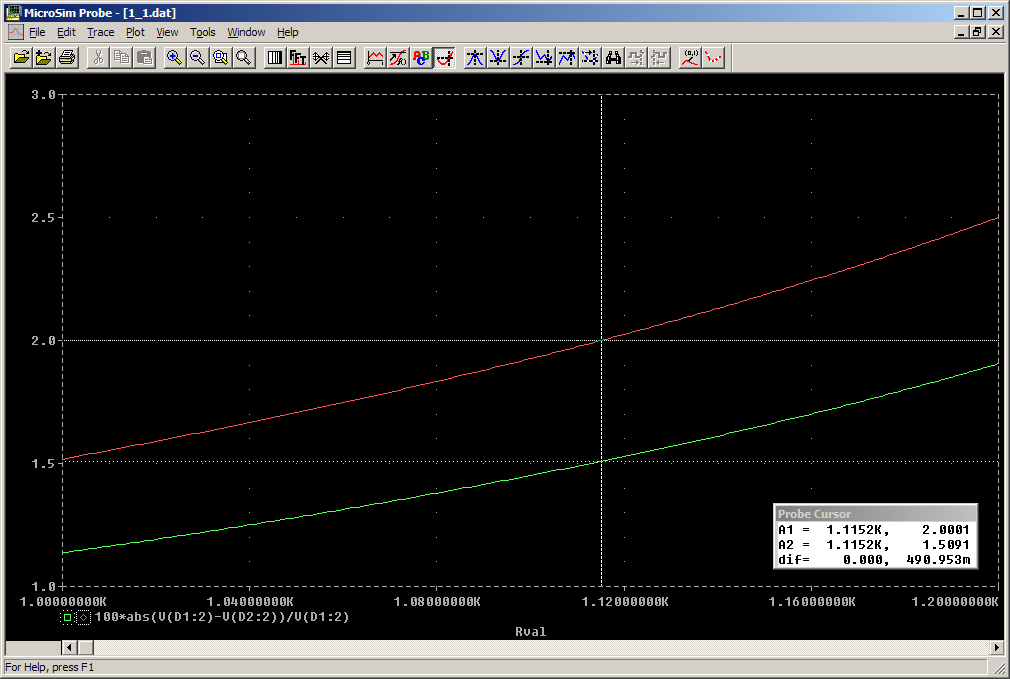
\includegraphics[width=\textwidth]{fig/bsp1/3_1_1_r1detail.PNG}
	\caption{Abweichung der Ausgangsspannungen f"ur feine Bestimmung von R1}
	\label{fig:3_1_1_r1detail}
\end{figure}


\subsection{Ausgangsspannungsschwankungen}

Zur Simulation der Schwankungen der Ausgangsspannungen wurde ein Breakout-Modell des Widerstands mit dem angegebenen Temperaturkoeffizienten verwendet. Um die Bauteiltoleranz zu ber"ucksichtigen wurde ein Parametric Sweep von R1 durchgef"uhrt, der den Idealwert des Bauteils und die maximalen Abweichungen (1\% bei E96) abdeckt. Abbildung~\ref{fig:3_1_2_e96dc} zeigt die entstehenden Bereiche wieder f"ur die Extremwerte der Temperatur.

\begin{figure}%[h!]
	\centering
	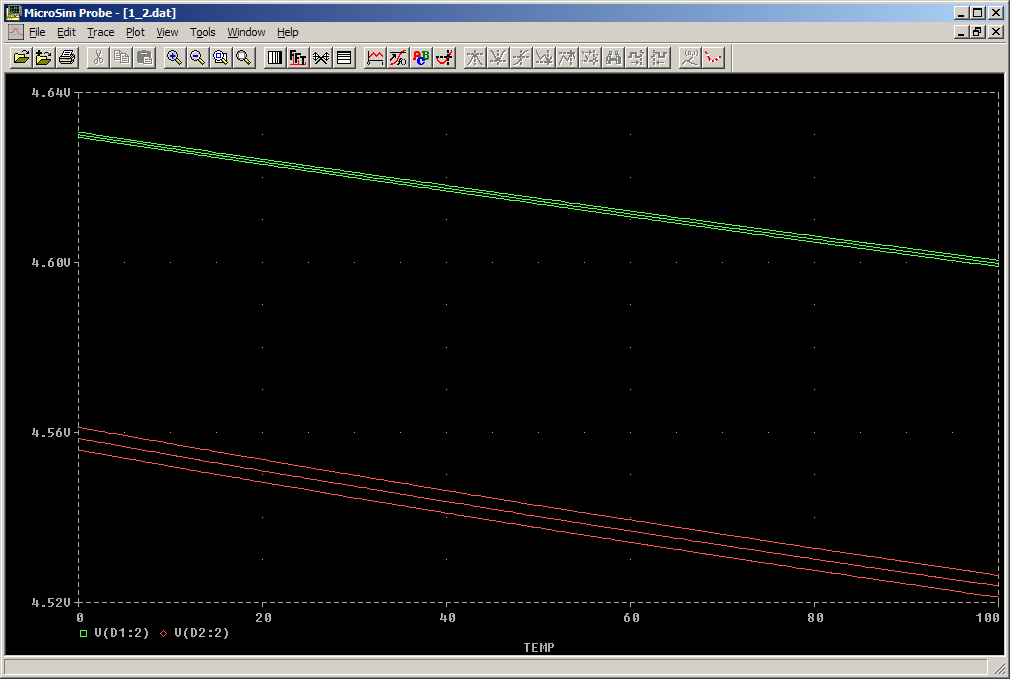
\includegraphics[width=\textwidth]{fig/bsp1/3_1_2_e96dc.PNG}
	\caption{Simulation der Toleranzen und Temperaturabh"angigkeit von R1}
	\label{fig:3_1_2_e96dc}
\end{figure}


\subsection{Ausgangswiderstand}

Zur Ermittlung des differentiellen Ausgangswiderstands ($r_a = \frac{du_a}{di_a}$) wurde mit einem DC Sweep der Laststrom variiert und mit einem Parametric Sweep die Versorgungsspannung im angegebenen Bereich variiert (f"ur eine Temperatur von 27 Grad). Abbildung~\ref{fig:3_1_3_ra} zeigt den Ausgangswiderstand "uber einen gro\ss{}en Bereich der Versorgungsspannung, Abbildung~\ref{fig:3_1_3_radetail} zeigt den Ausgangswiderstand in einem Bereich um den Arbeitspunkt von 3mA. Die gelbe Kurve stellt jeweils den Wert f"ur eine Versorgung mit 10V dar (Nominalwert).

\begin{figure}%[h!]
	\centering
	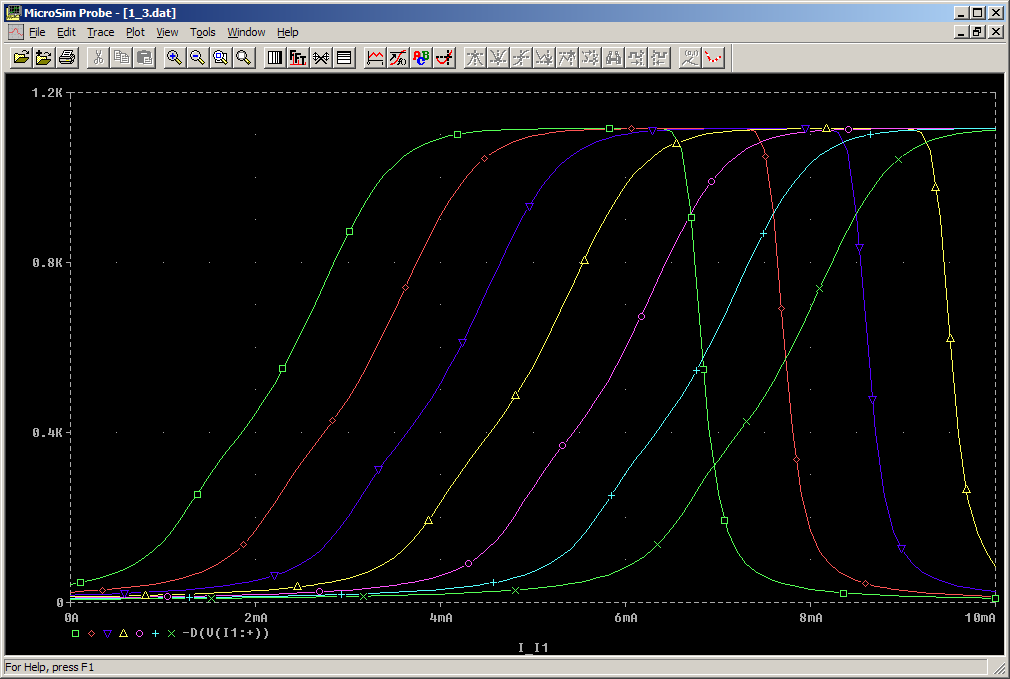
\includegraphics[width=\textwidth]{fig/bsp1/3_1_3_ra.PNG}
	\caption{Verlauf des differentiellen Ausgangswiderstands "uber gr"o\ss{}en Lastbereich}
	\label{fig:3_1_3_ra}
\end{figure}

\begin{figure}%[h!]
	\centering
	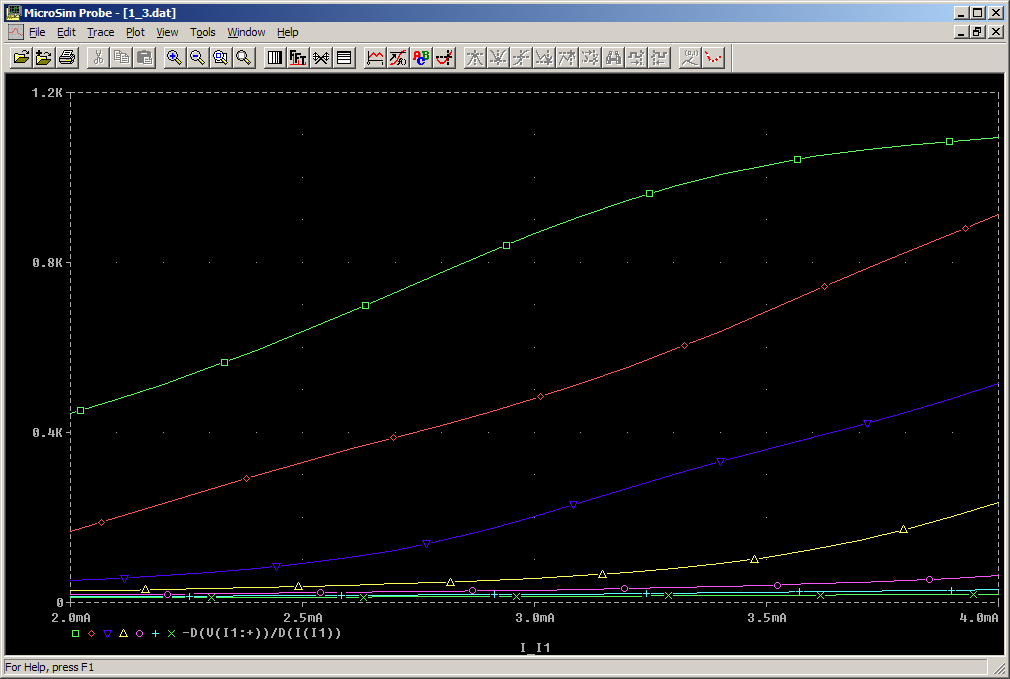
\includegraphics[width=\textwidth]{fig/bsp1/3_1_3_radetail.PNG}
	\caption{Verlauf des differentiellen Ausgangswiderstands um den Arbeitspunkt}
	\label{fig:3_1_3_ra}
\end{figure}



\section{Beispiel 2: RC-Bandpass}

\subsection{Ermittlung von R}

Zur Ermittlung von R wurde ein AC Sweep erstellt, der die Ausgangsspannung f"ur eine Frequenz (die Mittenfrequenz von 100kHz) simuliert. Zus"atzlich wurde mit einem Parametric Sweep R variiert. Der Spitzenwert entspricht dabei dem Widerstand, bei dem die Amplitude bei der Mittenfrequenz von 100kHz am h"ochsten ist. Abbildung~\ref{fig:3_2_1_rgrob} zeigt den Verlauf f"ur unterschiedliche R. Man erkennt, dass die Spitze zwischen $50\Omega$ und 100$\Omega$ liegt. Abbildung~\ref{3_2_1_rdetail} zeigt diesen Ausschnitt im Detail. Mit einem Cursor wurde der Maximalwert bei $72\Omega$ bestimmt. Dieser Wert stimmt mit dem errechneten Wert "uberein ($f_g = \frac{1}{2 \pi R C}$), und auch die Amplitude stimmt mit der Theorie "uberein ($\frac{V_{in}}{3}$).

\begin{figure}%[h!]
	\centering
	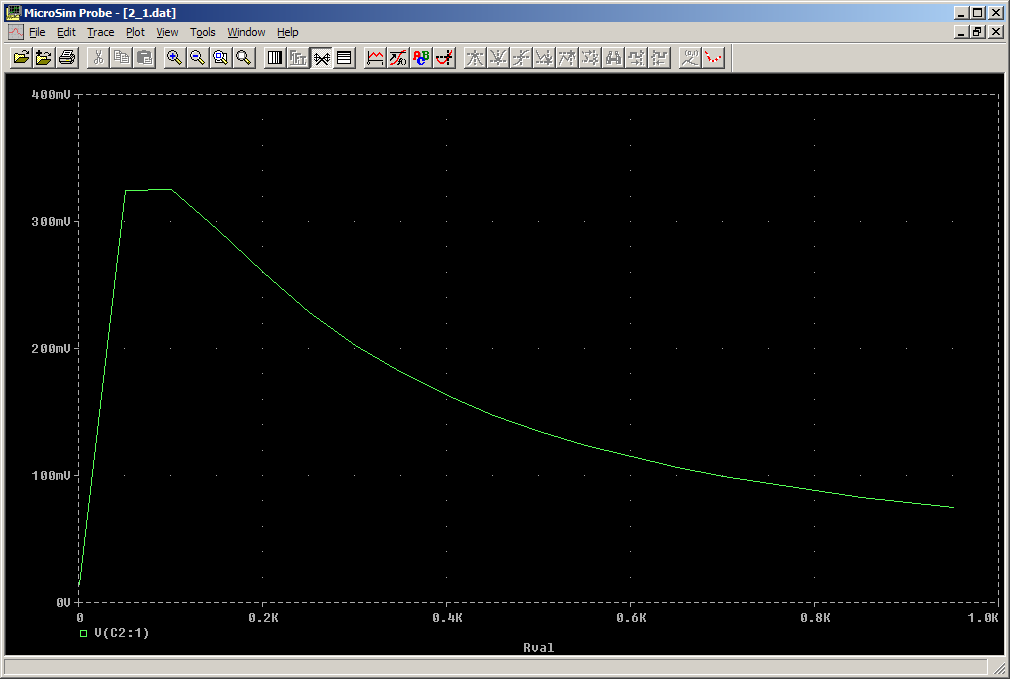
\includegraphics[width=\textwidth]{fig/bsp2/3_2_1_rgrob.PNG}
	\caption{Ermittlung von R "uber gro\ss{}en Widerstandsbereich}
	\label{fig:3_2_1_rgrob}
\end{figure}

\begin{figure}%[h!]
	\centering
	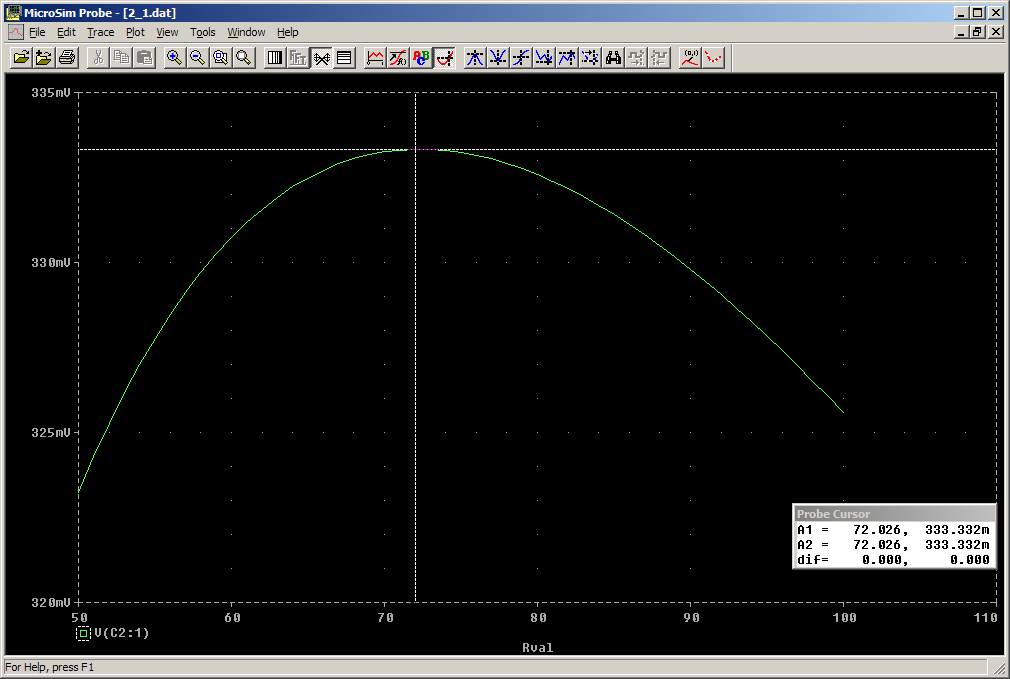
\includegraphics[width=\textwidth]{fig/bsp2/3_2_1_rdetail.PNG}
	\caption{genaue Ermittlung von R}
	\label{fig:3_2_1_rdetail}
\end{figure}

Zum "Uberpr"ufen wurde der Frequenzgang des Bandpasses f"ur die nominelle Temperatur und die Extremwerte der Temperaturen mittels AC Sweep simuliert (siehe Abbildung~\ref{fig:3_2_2_fT}). Bei 27 Grad ist die Mittenfrequenz genau 100kHz.

\begin{figure}%[h!]
	\centering
	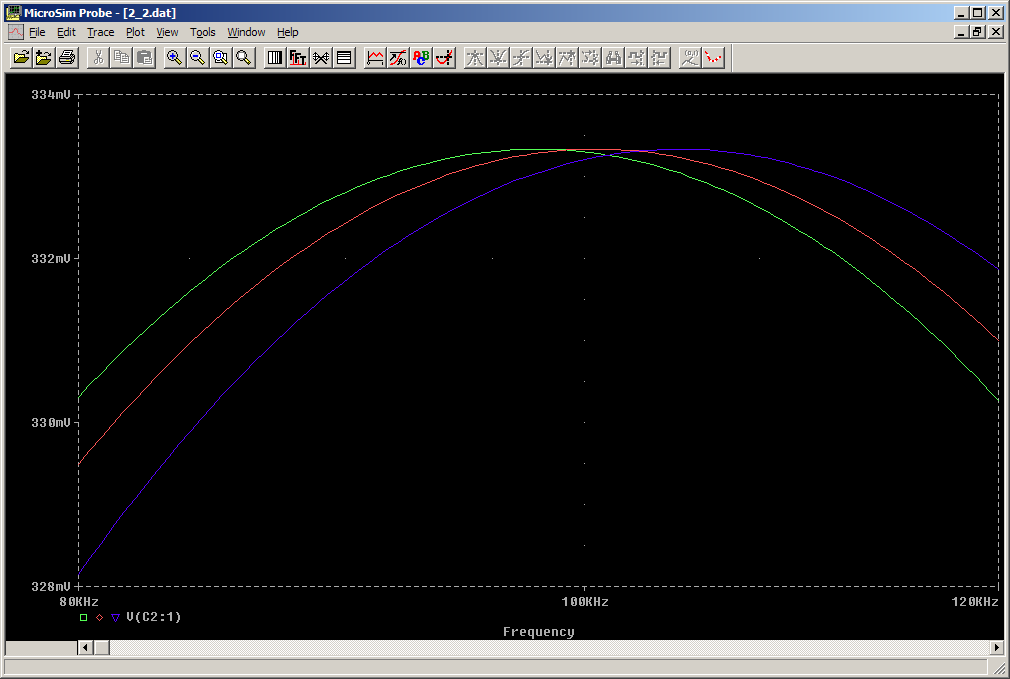
\includegraphics[width=\textwidth]{fig/bsp2/3_2_2_fT.PNG}
	\caption{"Uberpr"ufung der Funktion des RC-Bandpasses mit ermitteltem R}
	\label{fig:3_2_2_fT}
\end{figure}


\subsection{Worst Case Analyse}

Mit der Worst Case Analyse lassen sich die obere und untere Grenze f"ur die Ausgangswerte ermitteln, indem die schlechteste Kombination der toleranzbehafteten Bauteilwerte eingesetzt wird. Abbildung~\ref{3_2_2_wc_fT_both} zeigt die Simulation des nominalen Verhaltens (Mitte) und der Worst Cases (Minimum und Maximum) wieder bei den 3 Werten f"ur die Temperatur. Die Cursor markieren jeweils die entstehenden Mittenfrequenzen.

\begin{figure}%[h!]
	\centering
	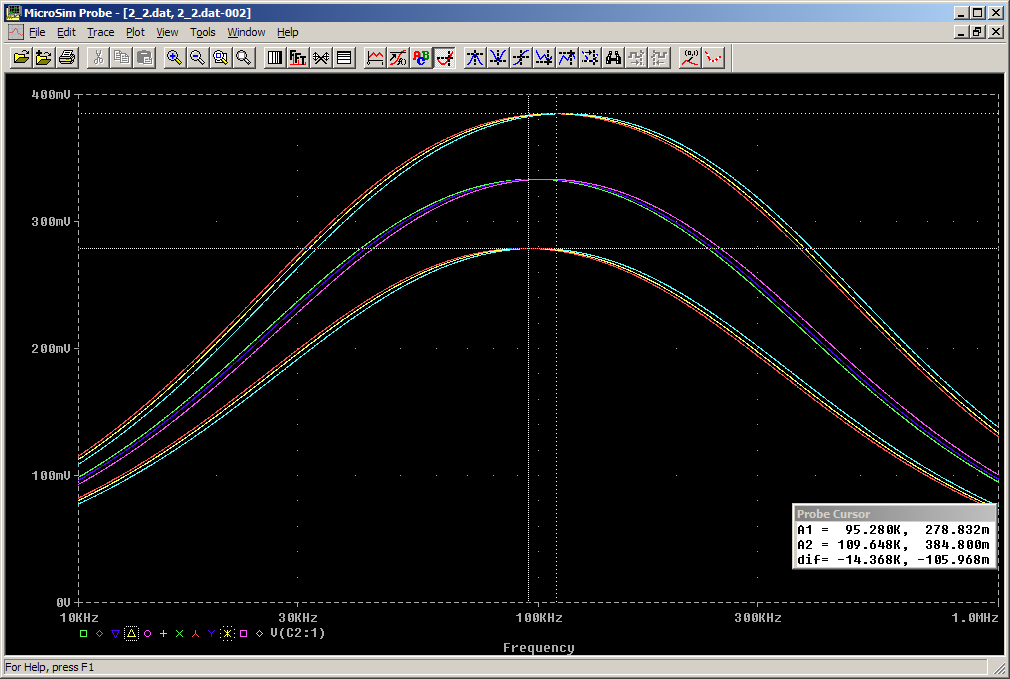
\includegraphics[width=\textwidth]{fig/bsp2/3_2_2_wc_fT_both.PNG}
	\caption{Worst Case Analyse f"ur toleranzbehaftete Bauteile}
	\label{fig:3_2_2_wc_fT_both}
\end{figure}

Die \emph{dev}-Toleranz entspricht dabei den Toleranzen der individuellen Bauteilen (jedes Bauteil f"ur sich), die \emph{lot}-Toleranzen entsprechen Toleranzen, die jeweils die Bauteile aus einer Charge gemeinsam haben. Dementsprechend ist es sinnvoll, bei einzeln gew"ahlten diskreten Bauteilen die \emph{dev}-Toleranz zu verwenden, und bei abgestimmten Bauteilen (z.B. Transistoren, Widerstandsarrays, etc) bzw. Bauteilen, die innerhalb einer Charge nur eine geringe Streuung aufweisen die \emph{lot}-Toleranz zu verwenden.


\subsection{Monte Carlo Analyse}

Mit der Monte Carlo Analyse lassen sich nicht die Extremwerte (Worst Cases), sondern statistische Schwankungen der Bauteile untersuchen. F"ur jeden Durchlauf werden Bauteilwerte innerhalb der Toleranzen zuf"allig gew"ahlt, mit denen dann die Schaltung simuliert wird. Die Darstellung ist als Kurvenschar oder als Histogramm m"oglich.

Abbildung~\ref{fig:3_2_2_mc_fT} zeigt eine Monte Carlo Analyse mit 3 Durchl"aufen f"ur die bereits aufgef"uhrten Temperaturen (aufgrund der geringen Anzahl an Durchl"aufen ist diese zwar nicht besonders aussagekr"aftig, aber gut ablesbar). Abbildung~\ref{fig:3_2_2_wc_mc} zeigt das Ergebnis einer Monte Carlo Analyse mit 10 Durchl"aufen, "uberlagert mit den Worst Case Werten. Man erkennt, dass die Monte Carlo Durchl"aufe innerhalb der Worst Cases liegen.

\begin{figure}%[h!]
	\centering
	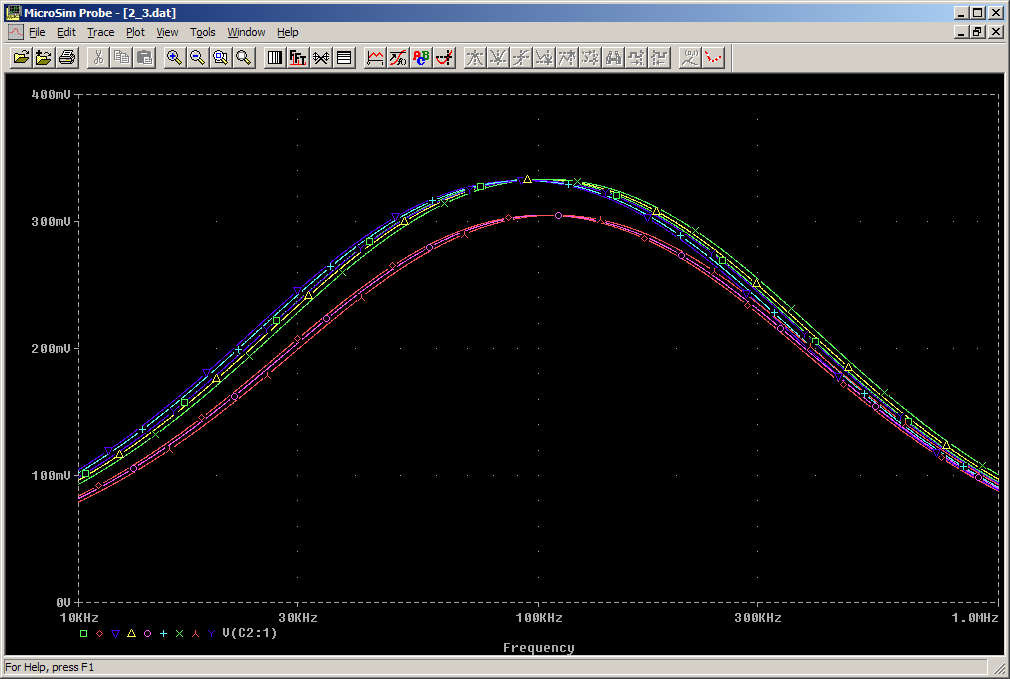
\includegraphics[width=\textwidth]{fig/bsp2/3_2_2_mc_fT.PNG}
	\caption{Monte Carlo Analyse f"ur toleranzbehaftete Bauteile (3 Durchl"aufe)}
	\label{fig:3_2_2_mc_fT}
\end{figure}

\begin{figure}%[h!]
	\centering
	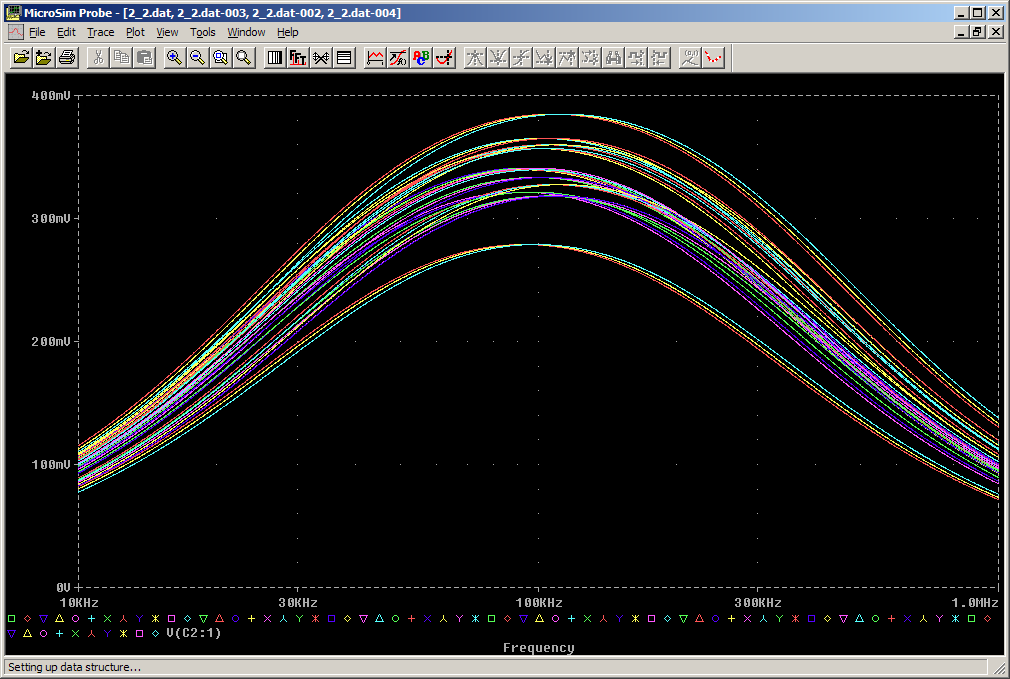
\includegraphics[width=\textwidth]{fig/bsp2/3_2_2_wc_mc.PNG}
	\caption{Monte Carlo Analyse f"ur toleranzbehaftete Bauteile (10 Durchl"aufe) "uberlagert mit Worst Cases}
	\label{fig:3_2_2_wc_mc}
\end{figure}

